

% ============================================================
%  NWU Faculty of Engineering – Final Year Project Report
%  main.tex  |  Top-level file
%
%  COMPILE:  pdflatex → biber → pdflatex → pdflatex
%            (or simply run:  latexmk -pdf main)
%
%  FOLDER STRUCTURE expected:
%    main.tex
%    NWUStyle.sty
%    NWUBack.png          <- purple NWU banner image
%    img/                 <- all figures go here
%    bib/
%      MyBib.bib          <- your BibTeX references
%    content/
%      00_abstract.tex
%      01_introduction.tex
%      02_problem_analysis.tex
%      03_literature.tex
%      04_concept.tex
%      05_preliminary.tex
%      06_detailed.tex
%      07_implementation.tex
%      08_testing.tex
%      09_conclusion.tex
%      A_ai_usage.tex
%      B_risk_register.tex
%      C_additional.tex
% ============================================================

% ── Document class ──────────────────────────────────────────
\documentclass[12pt, a4paper]{report}

\usepackage{NWUStyle} %You need the NWUStyle.sty file to be able to use this command.
 \usepackage{indentfirst}
% Point biblatex at your .bib file
\addbibresource{bib/MyBib.bib}


%================================================================================

% ============================================================
%    EDIT THESE FIELDS FOR YOUR PROJECT  
% ============================================================
 
% Full project title (appears large on cover)
\Title{Test Strength of 3D Printed Gears for Use in Pulley System Gearbox}
 
% Subtitle / report descriptor (leave blank with {} if unused)
\ReportTitle{Checkpoint 1 Report}
 
% Author
\Initials{J}
\FirstName{Juan}
\Surname{Fourie}
\StudentNumber{50128523}
 
% Supervisor(s) – leave blank with {} if unused
\Supervisor{Prof Henri Marais}
\CoSupervisor{}           % leave {} if none
\AssistantSupervisor{}    % leave {} if none
 
% ORCID – uncomment \showorcidtrue below and fill in number
\ORCID{0000-0000-0000-0000}
%\showorcidtrue            % uncomment to display ORCID on cover
 
% Degree information
\Degree{Bachelor of Engineering}
\Discipline{Mechatronic Engineering}
\Campus{Potchefstroom Campus}
 
% Module / assignment (for coursework reports – leave {} for FYP)
\Module{MCTR327}
\Assignment{Checkpoint 1}
 
% Dates
\Date{19 September 2026}       % generic date field
\SubmissionDate{19 September 2026}
 
% Turnitin score (leave {} to omit the line)
\TurnitinScore{}
 
% ============================================================

\begin{document}

% ── Cover page ──────────────────────────────────────────────
\MakeTitle
 
% ── Abstract + Keywords ─────────────────────────────────────
%\input{content/00_abstract}
 
% ── Table of Contents / List of Figures / List of Tables ────
\MakeTOCandLOFandLOT
 
% ── Declaration of Originality ──────────────────────────────
%\MakeDeclaration
 
% ── Switch to arabic page numbers for the body ──────────────
\cleardoublepage
\pagestyle{fancy}
\pagenumbering{arabic}
\setcounter{page}{1}
 
%================================================================================
%BEGIN TYPING YOUR DOCUMENT - STARTING HERE.-------------------------------------
%================================================================================

%EACH CHAPTER IS TYPED IN A SEPARATE FILE. YOU CAN ADD EACH FILE INTO YOUR DOCUMENT USING THE \input COMMAND.
% MAKE SURE THE FILES ARE IN THE SAME FOLDER AS THIS MAIN FILE.

% \input{content/ExampleChapter1} %Include the contents of the file "ExampleChapter1.tex"
% \input{content/ExampleChapter2} %Include the contents of the file "ExampleChapter2.tex"
% \input{content/ExampleChapter3} %Include the contents of the file "ExampleChapter3.tex"

% ============================================================
%  CHAPTER 1 – INTRODUCTION
% ============================================================
\section{Introduction}
\label{sec:introduction}

This report documents the testing of FDM 3D printed gears to determine their suitability in the construction of a gearbox for a gear pulley system.

\section{Experimental Setup}{}
\label{sec:experimental_setup}

\par
The following equipment was used in the experiment:
\begin{itemize}
    \item Load Cell
    \item Instrotech Model 4004 Load Cell Interpreter
    \item FDM 3D Printer
    \item PLA and PETG filament calibrated to filament roll
    \item Test Rig
    \item Jupyter and Latex
    
\end{itemize}


\begin{figure}[H]
    \centering
        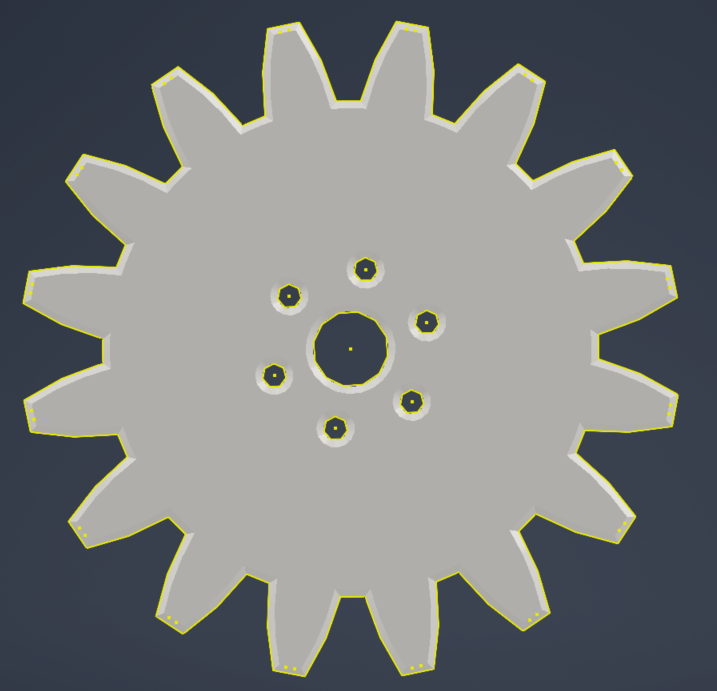
\includegraphics[width=0.75\textwidth]{img/im_gearDesignTested.png}
        \caption{Gear Design that was Tested}
        \label{im:geardesignTested}
\end{figure}

\par
A gear was designed to interface with the test rig in figure [\ref{im:testRigCAD}]. This rig uses a module 5 gear of 19mm diameter with 16 teeth and a 10mm diameter shaft hole. It has been designed with a 1mm chamfer to prevent elephant's foot while printing. It has 6 3.25mm holes for mounting screws to the flanges of the test rig. The printer has a tolerance of 0.2mm for printing in PLA and 0.3mm for PETG \cite{article_TonerPlastics}. The designed gear can be seen in figure [\ref{im:geardesignTested}].

\begin{figure}[H]
    \centering
        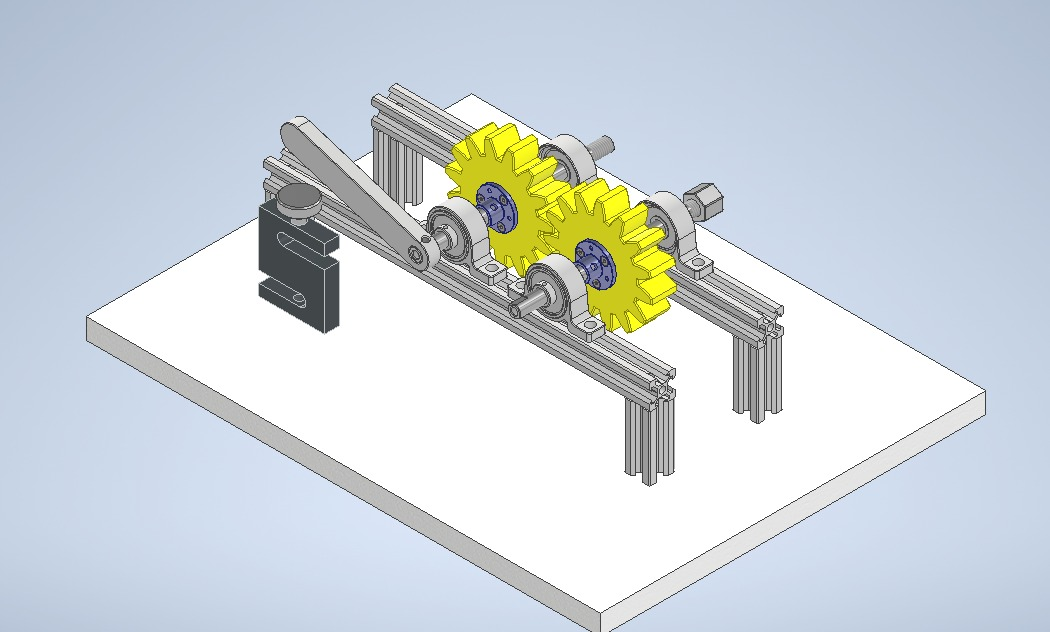
\includegraphics[width=0.75\textwidth]{img/im_testRigCAD.jpg}
        \caption{CAD Design of Rig Used to Test Gear Strength}
        \label{im:testRigCAD}
\end{figure}

\par
One gear was printed with PLA and the other with PETG. Each roll was calibrated beforehand and the relevant settings were applied. The gears were set to print with the specifications in table [\ref{tab:printsettings}]. Five layers all round are used for minimum material and maximum strength. A module five gear of this size has larger teeth than normal and if 3D printed it would have been best to print them with enough walls for solid gear teeth. This would however have increased material useage and print time with about 15 walls needed to completely fill the teeth. To compensate for this the gyroid infill setting was used to provide enough strength and general infill so that each tooth has the greatest chance of having the same strength compared to other infill settings \cite{youtube_LetsPrint}. The brim setting was used to ensure bed adhesion [\ref{im:gearSlicerSettings}]. The printed gears are shown in figure [\ref{im:2printedGears}].

\begin{table}[H]
    \centering
    \caption{Print Settings of printed gears}
    \label{tab:printsettings}
    \begin{tabular}{@{} l c @{}}
        \toprule
        \textbf{Parameter} & \textbf{Value} \\
        \midrule
        Wall Number & Value \\
        Bottom Shell Number & 5 \\
        Top Shell Number & 5 \\
        Infill Type & Gyroid \\
        Infill \% & 15 \% \\
        Brim & Outer Brim Only \\
        \bottomrule
    \end{tabular}
\end{table}

\begin{figure}[H]
    \centering
        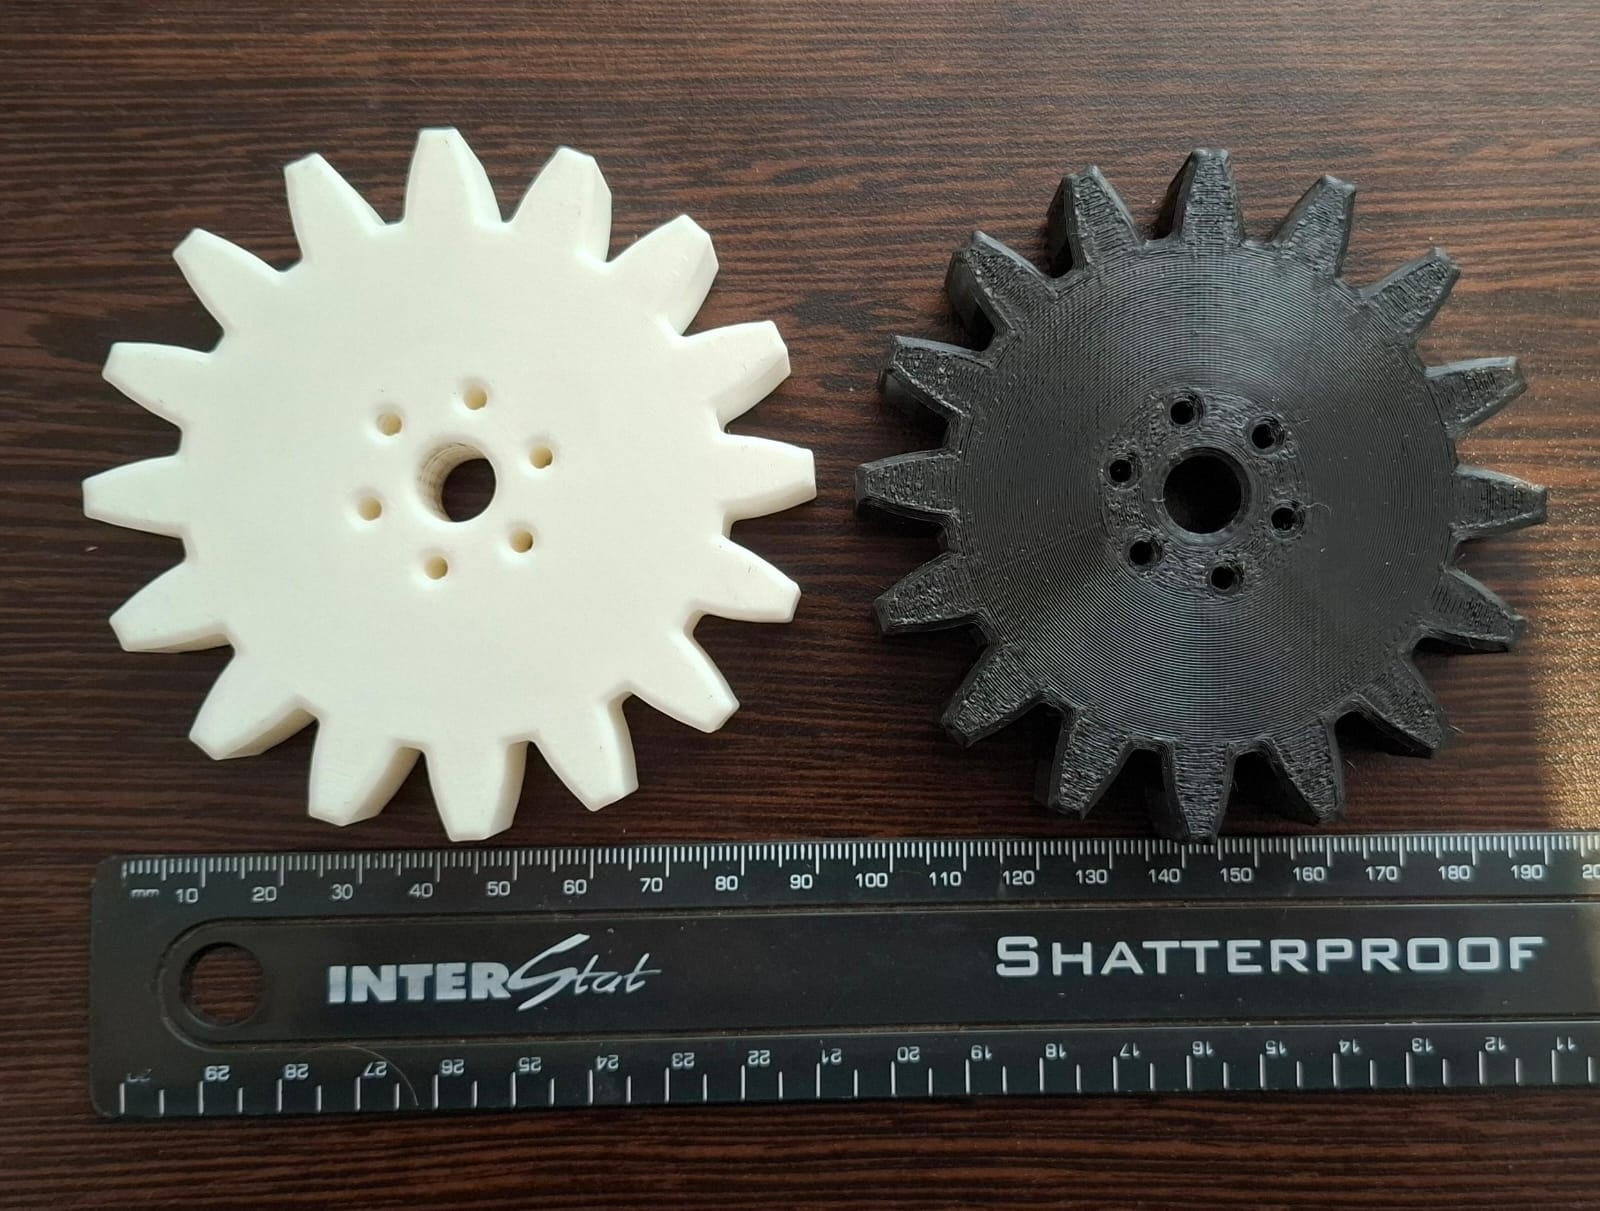
\includegraphics[width=0.75\textwidth]{img/im_2printedGears.jpeg}
        \caption{Image of the 2 Printed Gears. (White = PLA; Black = PETG)}
        \label{im:2printedGears}
\end{figure}


\begin{figure}[H]
    \centering
        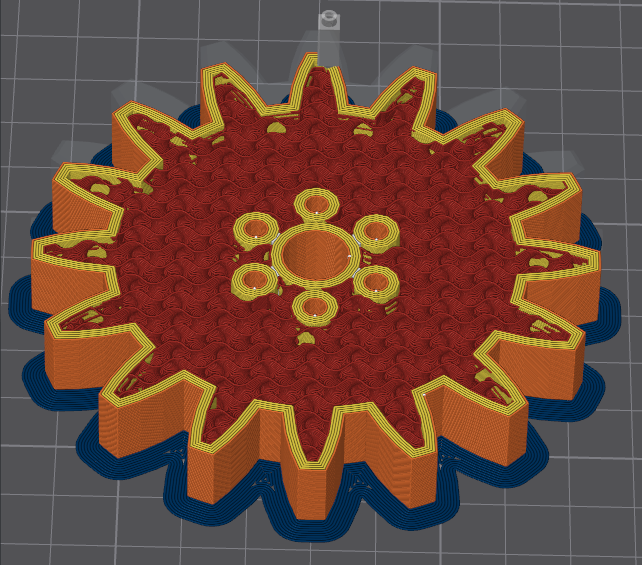
\includegraphics[width=0.75\textwidth]{img/im_gearSlicerSettings.png}
        \caption{Display of the internal slicer}
        \label{im:gearSlicerSettings}
\end{figure}




\section{Method}
\label{sec:method}

\par
The gears are to interface with the provided gear mounted on the test rig. A wrench would be attached to the one arm of the rig and turned to apply torque to the gears in the rig and subsequently to the arm applying the load to the load cell. The program interfacing with the Instrotech Model 4004 is set to start recording and the torque is applied until failure or the maximum load of 100 kg is applied to the load cell. The recorded results are exported as a .csv file and processed [\ref{im:testRig}].

\begin{figure}[H]
    \centering
        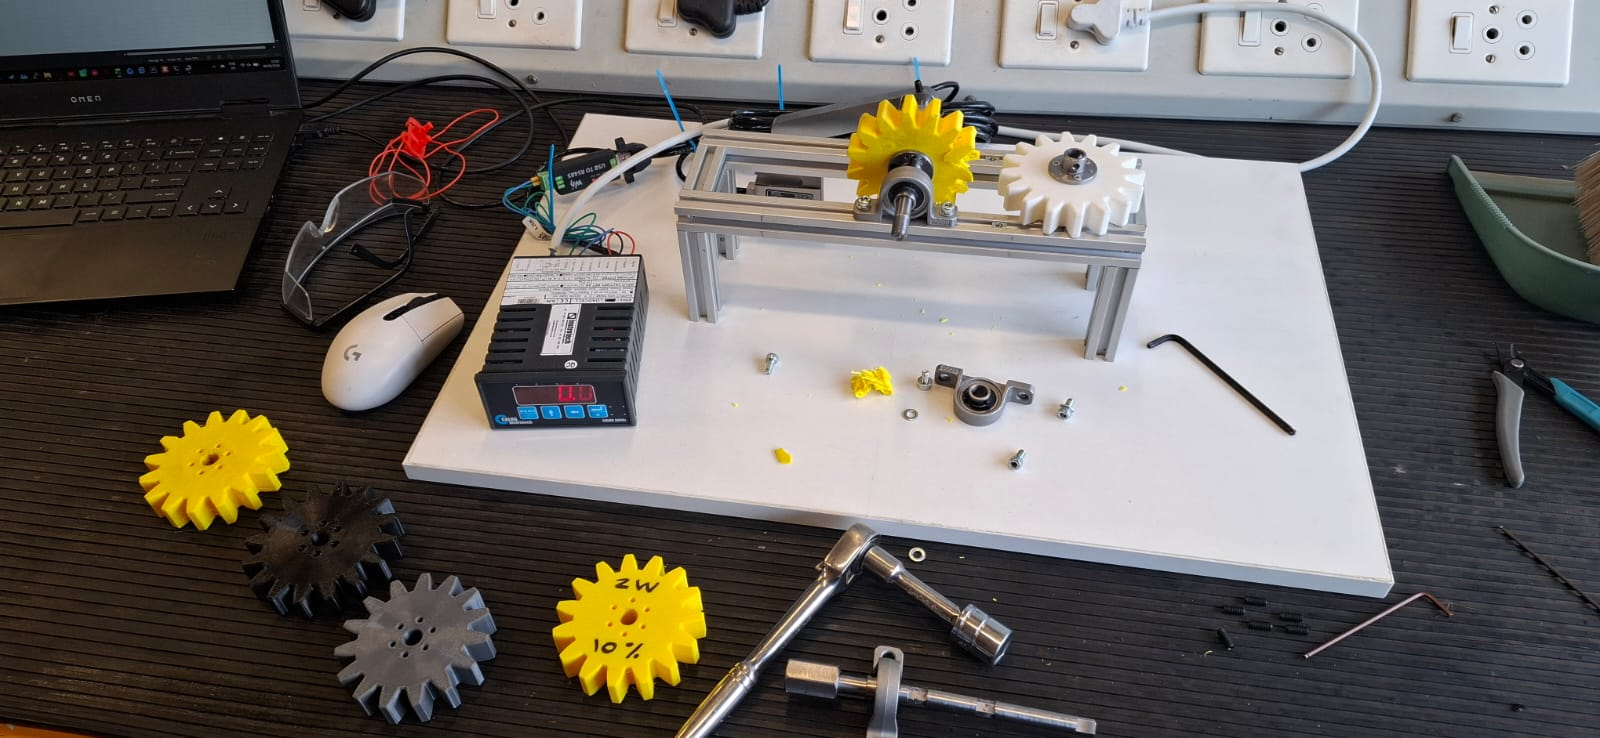
\includegraphics[width=0.75\textwidth]{img/im_testRig.jpeg}
        \caption{Rig Used to Test Gear Strength}
        \label{im:testRig}
\end{figure}

\par
To determine the results desired from the experiment, the following calculations and assumptions were made. A drum that has a height of 60mm and a diameter of 50mm was chosen. These were chosen so that the number of cable or rope can fit into only 1 wrap on the drum if the stroke is to be 1600mm if the rope were assumed to be 5mm in diameter. A mass of 30kg was assigned as the load of the drum at any one time to include the 20kg load with the equipment that might hang below it along with overhead. If the nominal speed of the motor is acheived at a speed of 1360 rpm with power of 0.18kW, then the gears need to withstand approximately 11,036Nm [\ref{eq:drum_torque}] if one is to withstand the maximum torque of the drum at any one time. It is unlikely that this top speed will be achieved by the motor due to the VFD limitations so these specifications will be prone to change [\ref{app:A_excel}].

\[
\tau_{\mathrm{Drum}} = \mathrm{Load} \times 9.81 \times \frac{\varnothing_{\mathrm{Drum}}}{2 \times 1000} \times K_{\mathrm{Serving\ Factor}}
\]

\par
Using the maximum load from the results, the torque applied to the gear can be determined and compared to the required torque. The test rig arm pressing onto the load cell is 100mm long[\ref{eq:rig_torque}].
\[
    \tau = F \times d
\]

\section{Results}
\label{sec:results}

\par
The results from the rig are rather the strength of the rig rather than that of the gears tested. The yellow gears in figure [\ref{im:testRig}] had failed before the loaded white and black gears. The PETG gear was used as the test gear agains the PLA gear. In this configuration the shaft failed as can be seen in figure [\ref{im:rigFailure}]. The results are however still usable.

\par
From the maximum load result of 16.8kg from the second PLA test, it can be calculated that the torque is 16.68Nm [\ref{eq:rig_torque}]. 
\[
    \tau = F \times d
    \]
    \[   
    \tau = 16.8 \times 9.81 \times 0.01 
    \]
    \[
    \tau = 16.68\,\mathrm{Nm}
\]
    

\begin{figure}[H]
    \centering
        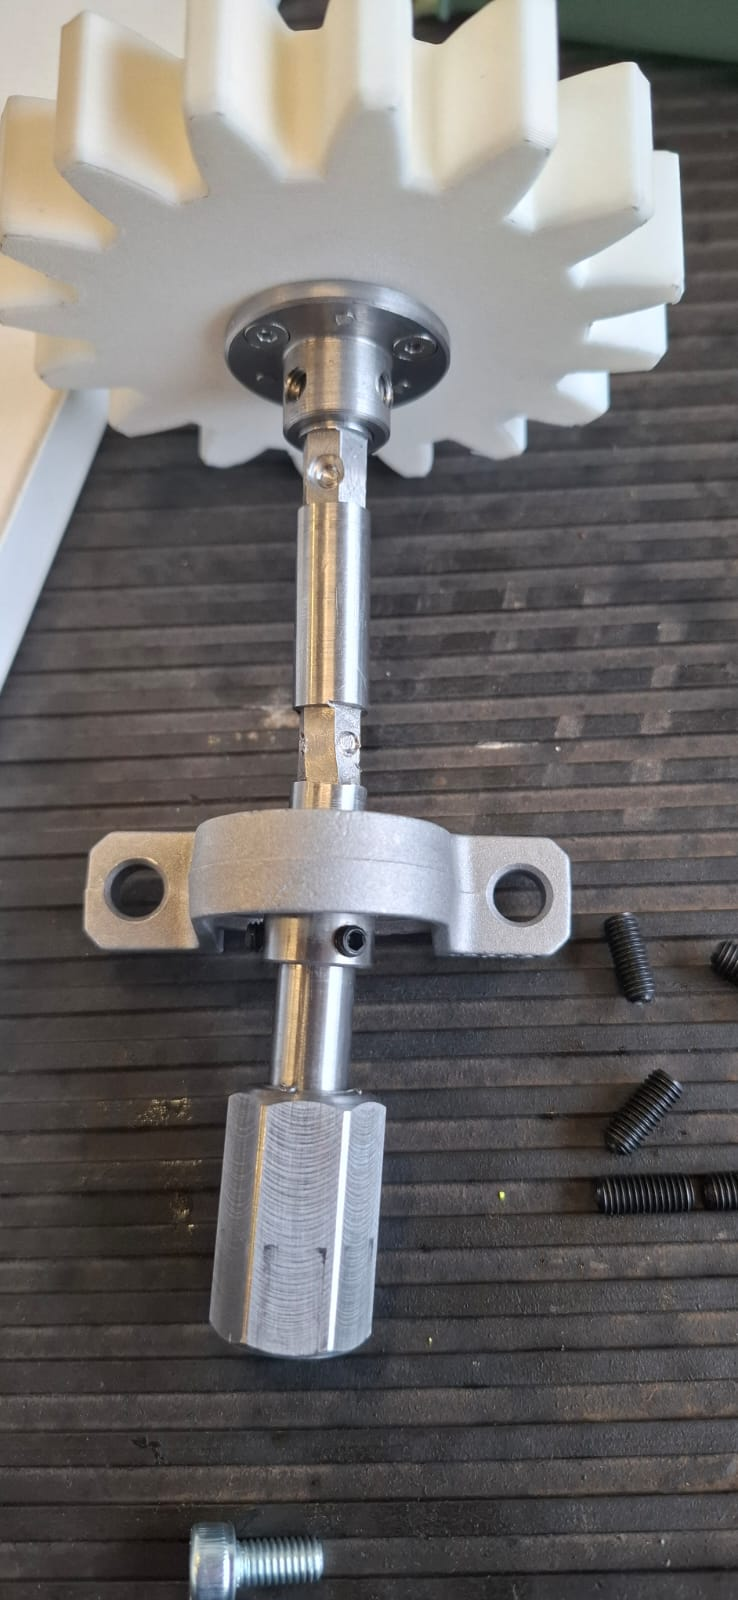
\includegraphics[width=0.5\textwidth]{img/im_rigFailure.jpeg}
        \caption{Rig Failure During Test}
        \label{im:rigFailure}
\end{figure}


\begin{figure}[H]
    \centering
        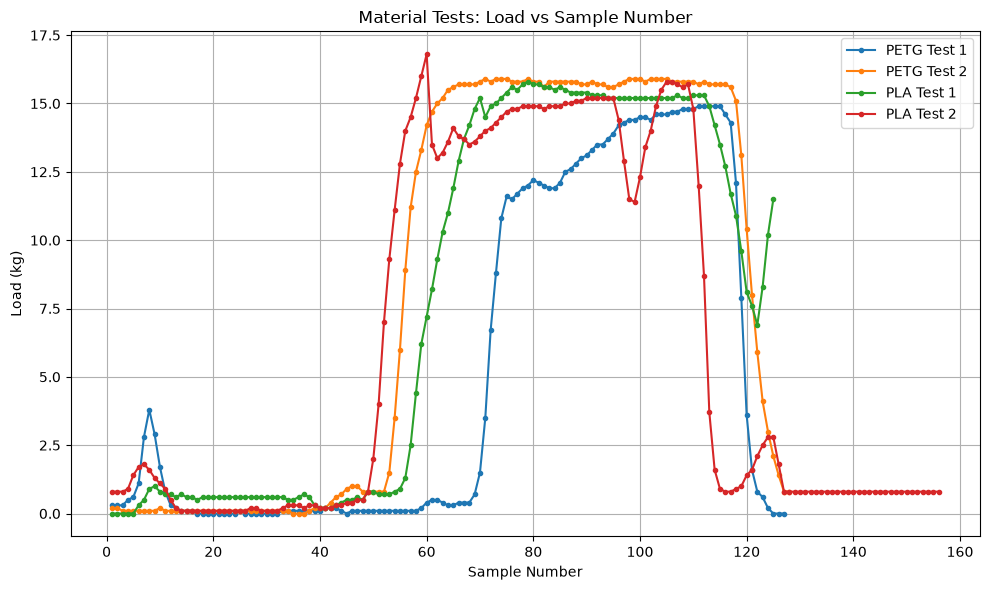
\includegraphics[width=1\textwidth]{figures/chart_loadvssamplenumber.png}
        \caption{Results of the gears tested}
        \label{ch:loadvssamplenumber}
\end{figure}
\section{Discussion}
\label{sec:discussion}

\par
From the results seen in figure [\ref{ch:loadvssamplenumber}], it can be seen that the maximum load carried by the rig gears before gear or shaft failure of the rig was around 17kg for the second PLA gear test. Both the PLA and PETG gears seen in figure [\ref{im:2printedGears}] had not failed, implying they will be able to withstand even greater loads.

\par
The mounting options for the gears to the shafts will need to be tested as well \cite{youtube_LetsPrint} \cite{textbook_Shigley}. The gears used in the gearbox will also be of a smaller module, and thickness to be adhere to space limitations on the rig.
\section{Conclusion}
\label{sec:conclustion}

\par
The gears tested will be able to bear the load necessary if one gear were to be bear all the torque of the entire load. This has been concluded as unlikely and since the gears of the test rig failed, the implication is that the tested gears will be able to withstand even greater loads. The poorly printed gears withstood 16.68Nm of torque while the requirement is only 11Nm The final gears to be used in the gearbox will however also be tested before final implementation to also test whether the gear mounting option chosen is sufficient.


% ── References ──────────────────────────────────────────────
 \newpage
 \printbibliography[heading=bibintoc, title={References}]
 
% ── Appendices ──────────────────────────────────────────────
\newpage
\appendix
\appendix
\section{Appendix A: Excel Tables for Calculations}
\label{app:A_excel}

% Table generated by Excel2LaTeX from sheet 'Sheet1'
\begin{table}[H]
  \centering
  \caption{Design main specifications}
  \begin{tabular}{|r|r|l|}
    \hline
    \multicolumn{3}{|c|}{\textbf{Design Main Specifications}} \\
    \hline
    \multicolumn{1}{|l|}{Max Load} & 30 & kg \\
    \multicolumn{1}{|l|}{Stroke} & 1600 & mm \\
    & 80 & mm/s \\
    \hline
  \end{tabular}
  \label{tab:design_main_specs}
\end{table}

% Table generated by Excel2LaTeX from sheet 'Sheet1'
\begin{table}[H]
  \centering
  \caption{Gear specifications}
  \begin{tabular}{|l|r|l|l|}
    \hline
    \multicolumn{4}{|c|}{\textbf{Gear Specs}} \\
    \hline
    \textbf{Parameter} & \textbf{Value} & \textbf{Unit} & \textbf{Comment} \\
    \hline
    Module & 2 & ul & \\
    Number\_of\_Teeth & 30 & ul & \\
    Pressure\_Angle & 25 & deg & \\
    Gear\_Height & 15 & mm & \\
    Pitch\_Circle & 60 & mm & \\
    Addendum\_Circle & 64 & mm & \\
    Root\_Circle & 55 & mm & \\
    Clearance\_Circle & 56 & mm & \\
    Base\_Circle & 54.37847 & mm & \\
    \hline
    Reduction Ratio & 44.5059 & & \\
    Per Stage work & 6.671274 & & \\
    Np & 11 & & \\
    Ng & 250 & & \\
    m & 22.72727 & & \\
    \hline
  \end{tabular}
  \label{tab:gear_specs}
\end{table}

% Table generated by Excel2LaTeX from sheet 'Sheet1'
\begin{table}[H]
  \centering
  \caption{Drum specifications}
  \begin{tabular}{|l|r|l|}
    \hline
    \multicolumn{3}{|c|}{\textbf{Drum Specs}} \\
    \hline
    Line Speed & 88 & mm/s \\
    Diameter & 50 & mm \\
    Height & 60 & mm \\
    Starting Serving Factor & 1,5 & \\
    Circumference & 157.0796 & mm \\
    Loops of Circ fitted & 12 & \\
    Rope Length in 1 layer & 1884.956 & \\
    Rpm & 30.55775 & \\
    Torque & 11.03625 & Nm \\
    \hline
  \end{tabular}
  \label{tab:drum_specs}
\end{table}

% Table generated by Excel2LaTeX from sheet 'Sheet1'
\begin{table}[H]
  \centering
  \caption{Rope specifications}
  \begin{tabular}{|l|r|l|}
    \hline
    \multicolumn{3}{|c|}{\textbf{Rope Specs}} \\
    \hline
    Diameter & 5 & mm \\
    Length & 1600 & mm \\
    Wraps & 10.18592 & \\
    \hline
  \end{tabular}
  \label{tab:rope_specs}
\end{table}

% Table generated by Excel2LaTeX from sheet 'Sheet1'
\begin{table}[H]
  \centering
  \caption{Three-phase motor specifications}
  \begin{tabular}{|l|r|l|}
    \hline
    \multicolumn{3}{|c|}{\textbf{3-Phase Motor Specs}} \\
    \hline
    Power & 0.18 & kW \\
    Speed & 1360 & rpm \\
    Mass & 4.83 & kg \\
    Shaft & 11 & mm \\
    Keyway & 4*16 & mm \\
    Rated Torque & 1.263877 & Nm \\
    Starting Torque & 3.791632 & Nm \\
    \hline
  \end{tabular}
  \label{tab:motor_specs}
\end{table}


\appendix
\section{Appendix B: Equations}
\label{app:B_equations}

\begin{equation}
\label{eq:drum_torque}
\tau_{\mathrm{Drum}} = \mathrm{Load} \times 9.81 \times \frac{\varnothing_{\mathrm{Drum}}}{2 \times 1000} \times K_{\mathrm{Serving\ Factor}}
\end{equation}

\begin{equation}
\label{eq:min_gear}
\mathrm{N_P} = \frac{2\mathrm{k}}{(1 + 2\mathrm{m})\sin^2 \phi} \left( \mathrm{m} + \sqrt{\mathrm{m}^2 + (1 + 2\mathrm{m})\sin^2 \phi} \right)\end{equation}

\begin{equation}
\label{eq:max_gear}
\mathrm{N_G} = \frac{\mathrm{N_P}^2 \sin^2 \phi - 4k^2}{4k - 2N_P \sin^2 \phi}
\end{equation}

\begin{equation}
\label{eq:pitch_circle}
D_P = \mathrm{module} \times \mathrm{z}
\end{equation}

\begin{equation}
\label{eq:gear_module}
\mathrm{D} = \frac{p}{\pi}
\end{equation}


\begin{equation}
\label{eq:addendum_circle}
D = D_p + 2 \times m
\end{equation}


\begin{equation}
\label{eq:root_circle}
D_r = D_p - 2 \times b
\end{equation}


\begin{equation}
\label{eq:dedendum}
b = 1.25 \times m
\end{equation}

\begin{equation}
\label{eq:clearance_circle}
D_c = D_p - 2\times m
\end{equation}


\begin{equation}
\label{eq:circular_pitch}
p = m\times\pi
\end{equation}

\begin{equation}
\label{eq:base_circle}
D_b = D_p \cos{\alpha}
\end{equation}

\begin{equation}
    \label{eq:rig_torque}
    \tau = F \times d
\end{equation}
% \input{content/C_additional}
 
\end{document}
